\subsection{Model specification and modeling assumptions}
\label{sec:modelspecificationandmodelingassumptions}

In this section, it is discussed how the specification of mixed models differs from that of fixed effects models, and that for each model with random effects there is an alternative models with only fixed effects.
It is based mostly on Part~2A of \citet{GelmanHill2006} (pp.~235--342).
% A major focus is on the question of when to use fixed and random effects.
% The amount of technicality and notation is kept at the absolute minimum, but a few notational conventions are introduced to enable readers to understand both the output of \texttt{lme4} and other packages in \texttt{R} as well as the literature on mixed models.
% To make successful practical use of mixed models, some level of fundamental understanding is required.

\subsubsection{Simple random intercepts}
\label{sec:simplerandomintercepts}

Readers with experience in fixed effects modeling should be able to see that a grouping factor encoding the verb lemma and all the other grouping factors discussed in the previous sections could be specified as a normal fixed effect in a GLM.
In such a case, each of the $m$ levels of the speaker factor is dummy-coded, and for all but one of these binary dummy variables, a coefficient is estimated.
Logistic regression examples are used throughout this section, and we begin with the fictional corpus study of the dative alternation introduced in Sections~\ref{sec:hierarchicalormultilevelmodels} and \ref{sec:randominterceptsandslopes}.
We first specify a minimal model with only the dummies of the lemma grouping factor and one other (binary) predictor, namely givenness.
There are $m$ verb lemmas (\ie groups) and $n$ observations.
As index variables, we use $j$ for groups and $i$ for observations.
In general, $\alpha$ is used for intercepts and $\beta$ for coefficients.
A specification of such a model is given in (\ref{eq:glm01}).

\begin{equation}
  Pr(y^i=1)=logit^{-1}(\alpha_0+\beta_d\cdot x_{d}^i+\beta_{l_1}\cdot x_{l_1}^i+\beta_{l_2}\cdot x_{l_2}^i+\cdots+\beta_{l_{m-1}}\cdot x_{l_{m-1}}^i)
  \label{eq:glm01}
\end{equation}

This models the estimate of the probability ($Pr$) that in observation $i$, the outcome variable $y^i$ is $1$, \ie that dative shift occurs.
$\alpha_0$ is the intercept, $\beta_d$ is the coefficient for the effect of givenness.
$x_d^i$ is the value of the variable that encodes givenness for exemplar $i$ ($0$ for discourse-old NPs and $1$ for discourse-new NPs).
Furthermore, $\beta_{l_j}$ are the coefficients for the lemma dummy variables.
Finally, $x_{l_j}^i$ is the value ($0$ or $1$) for lemma $j$ in observation $i$.
If in data point $64$, the lemma is \textit{give} and \textit{give} is encoded as group $12$, then $i=64$, $j=12$, and $x_{l_{12}}^{64}=1$, whereas all $x_{l_j}^{64}=0$ with $j\neq12$.
Because one verb lemma dummy variable is on the intercept $\alpha_0$ and thus used as a reference, we only estimate $m-1$ instead of $m$ coefficients, \ie $j=1,\cdots,m-1$.%
\footnote{Picking one dummy as a reference level is necessary because otherwise infinitely many equivalent estimates of the model coefficients exist because one could simply add any arbitrary constant to the intercept.
However, the estimator works under the assumption that there is a unique maximum likelihood estimate.
This extends to other possible encodings of the categorical grouping variable.}
The function $logit^{-1}$ is the \textit{link function}, and its argument is the \textit{linear term} of the model.
In such a model, the effect of each verb lemma is treated as a fixed population parameter, exactly the same as the effect of givenness.
% The coefficient $\beta_d$ is estimated in exactly the same way as each $\beta_{l_j}$.

If we treat the same grouping factor as a random intercept, we let the intercept vary by group.
In other words, each group is allowed to have its own intercept.
Furthermore, we give the varying intercepts a (normal) distribution instead of estimating $m-1$ coefficients.
In other words, the group-wise intercepts are assumed to be normally distributed, typically around $0$.
This is the relevant difference between a fixed effect and a random effect.
The model specification then looks like in (\ref{eq:glmm01}).

\begin{equation}
  P(y^i=1)=logit^{-1}(\alpha_{l}^{j[i]}+\beta_d\cdot x_d^i)
  \label{eq:glmm01}
\end{equation}

We now have an intercept $\alpha_l^{j[i]}$ which varies by group (instead of one term with its own coefficient per group).
We use the notation $\alpha_l^{j[i]}$ (borrowed in a modified form from \citealt{GelmanHill2006}) to indicate that the correct $j$-th lemma intercept is chosen for the $i$-th observation.
For example, if in exemplar $64$, the lemma is \textit{give}, which is group $12$, then $i=64$ and $j[64]=12$ (\ie the group appropriate for exemplar $64$ is group $12$), and $\alpha_l^{j[64]}=\alpha_l^{12}$.
The term $\beta_d\cdot x_d^i$ for the effect of givenness remains unchanged when going from (\ref{eq:glm01}) to (\ref{eq:glmm01}).
Crucially, instead of estimating a batch of coefficients for the lemma effect, $\alpha_l$ is itself modeled, and random terms are predicted for each level of the random effect.
For this, the assumption in (\ref{eq:glmm02}) is made.

\begin{equation}
  \alpha_l^j\sim N(\mu_l,\sigma_l^2)
  \label{eq:glmm02}
\end{equation}

This is standard notation to indicate that the values of $\alpha_l^j$ follow a normal distribution with mean $\mu_l$ and a variance of $\sigma_l^2$.
In fact, we can regard (\ref{eq:glmm02}) as a minimal second-level model already, although one which simply predicts varying intercepts from a normal distribution.
All more complex models to be discussed below are extensions of this approach.
In the next section, the consequences of going from a fixed effect to a random effect are discussed.

\subsubsection{Choosing between random and fixed effects}
\label{sec:choosingbetweenrandomandfixedeffects}

There are primarily two points to consider which influence the decision whether to use random effects.
First, the variance in the intercepts (and for random intercept-random slope models also the covariance between intercepts and slopes) needs to be estimated.
Second, the random intercepts can be understood as a compromise between fitting separate models for each group of the grouping factor (\textit{no pooling}) and fitting a model while ignoring the grouping factor altogether (\textit{complete pooling}), see \citet[Ch.~12]{GelmanHill2006}.
% While all conditions which were discussed in the previous chapter (independence of observations, non-collinearity, etc.) must also be met by hierarchical models, these two points add additional conditions.

As was stated above in (\ref{eq:glmm02}), the random intercepts are assumed to follow a normal distribution, and the variance $\sigma_l^2$ needs to be estimated with sufficient precision.
From the estimated variance and the data, the estimator then predicts the \textit{conditional modes} in GLMMs (\textit{conditional means} in LMMs) for each group (see \citealt[Ch.~1]{Bates2010}), which is the numerical value which software packages like \texttt{lme4} produce for each level of the grouping factor.
% , and these values are sometimes sloppily called ``random effects'' by practitioners.
This procedure, however, requires that the number of groups must not be too low to effectively achieve this.
As a rule of thumb, fewer than five levels means that a grouping factor should be included as a fixed effect, regardless of its conceptual nature.
Even if there is a default recommendation to use a speaker grouping variable as a random effect, it is ill-advised to do so if there are exemplars from less than five speakers in the sample.
Along the same lines, mode (typically spoken vs.\ written) is no suitable grouping factor for use as a random effect.
% Very often, the estimator will fail anyway under such conditions.
% Thus, a random effect might be the best option for technical reasons.

If, however, the number of groups is reasonably large, the next thing to consider is the number of observations per group.
Alternatives to using a random effect would be to estimate a separate model for each level of the grouping factor, or to include it as a fixed effect.
In both cases the effects are not treated as random variables, and fixed coefficients per group are estimated without taking the between-group variance into account.
% The estimation of coefficients for a (dummy-coded) fixed effect becomes less precise and feasible with large numbers of levels or when there are levels with very few observations.
With a random effect, however, the conditional modes\slash means are pulled (\textit{shrunken}) towards the overall intercept (\textit{shrinkage}).%
\footnote{Notice that \textit{mode} here refers to the statistical usage of the word.}
When there the number of observations in a group is low, the conditional mode\slash mean is simply shrunken more strongly towards $0$, predicting only a small deviation from the overall tendency.%
\footnote{Terminologically, shrinkage is thus \textit{stronger} and the conditional mode\slash mean is closer to $0$ for a specific group if there is less evidence that the group deviates from the overall tendency.
The lower the number of observations per group, the lesser evidence there is.}
Fixed effect estimates, on the other hand, become inexact and will probably be dismissed because of growing uncertainty in the estimate (large confidence intervals, non-significance) when the number of observations in a level is low.
Put differently, low numbers of observations in all or some groups are often detrimental for using fixed effects grouping factors.
Random effects can deal with situations like this much better because of shrinkage.
On the downside, a conditional mode that was strongly shrunken (due to a low number of observations) cannot be distinguished straightforwardly from a conditional mode of a group which simply does not deviate a lot from the average tendency.
For fixed effects, we have both a parameter estimate and a possible significance test, but for random effects, we only have the prediction of the conditional mode\slash mean.
Still, including a grouping factor as a random effect might be the only way of using it at all when the estimation as a fixed effect fails.

This section closes with an illustration.%
\footnote{The code for these and other simulations is available under a Creative Commons Attribution license: \url{https://github.com/rsling/Rstuff/tree/master/simulations/glmm}}
For this, 1,000 data sets were simulated which corresponded to the model in (\ref{eq:glmm03}) and (\ref{eq:glmm04}).
We drop the subscripts on $\alpha$, $\beta$, and $\mu$ for convenience since there is only one random intercept.

\begin{align}
  P(y^i=1) & =logit^{-1}(\alpha^{j[i]}+\beta_1\cdot x_1^i+\beta_2\cdot x_2^i)
  \label{eq:glmm03}\\
  \alpha^j & \sim N(\mu, \sigma)\label{eq:glmm04}
\end{align}

Again, this could be a model of a binary alternation such as the dative alternation.
$x_1$ is a binary variable (such as given\slash new) and $x_2$ a continuous variable (such as NP length).
Since the data were simulated, the parameters to be estimated are known: $\beta_1=0.8$, $\beta_2=-1.3$, $\mu=0$, $\sigma=1.5$.
The number of groups was set to $5$, and each group could correspond to a single writer or a specific verb lemma.
The simulated values of the grouping factor were identical in each simulation, and there were $20$ observations per group.
Figure~\ref{fig:glmmj5i20} shows the distribution of the group levels based on the conditional modes predicted of all but the first group in the $1,000$ simulations.
Figure~\ref{fig:glmj5i20} shows the group estimates from a model where the grouping factor was added as a fixed effect.%
\footnote{The plots do not show the distribution of the raw conditional modes and coefficient estimates of the fixed effects.
Rather, the overall intercept was taken into account, and the plots thus show the distribution of the per-group prediction of the models, all other things being equal.
This is what was pre-specified in the simulations.}

\begin{figure}[!htpb]
  \centering
  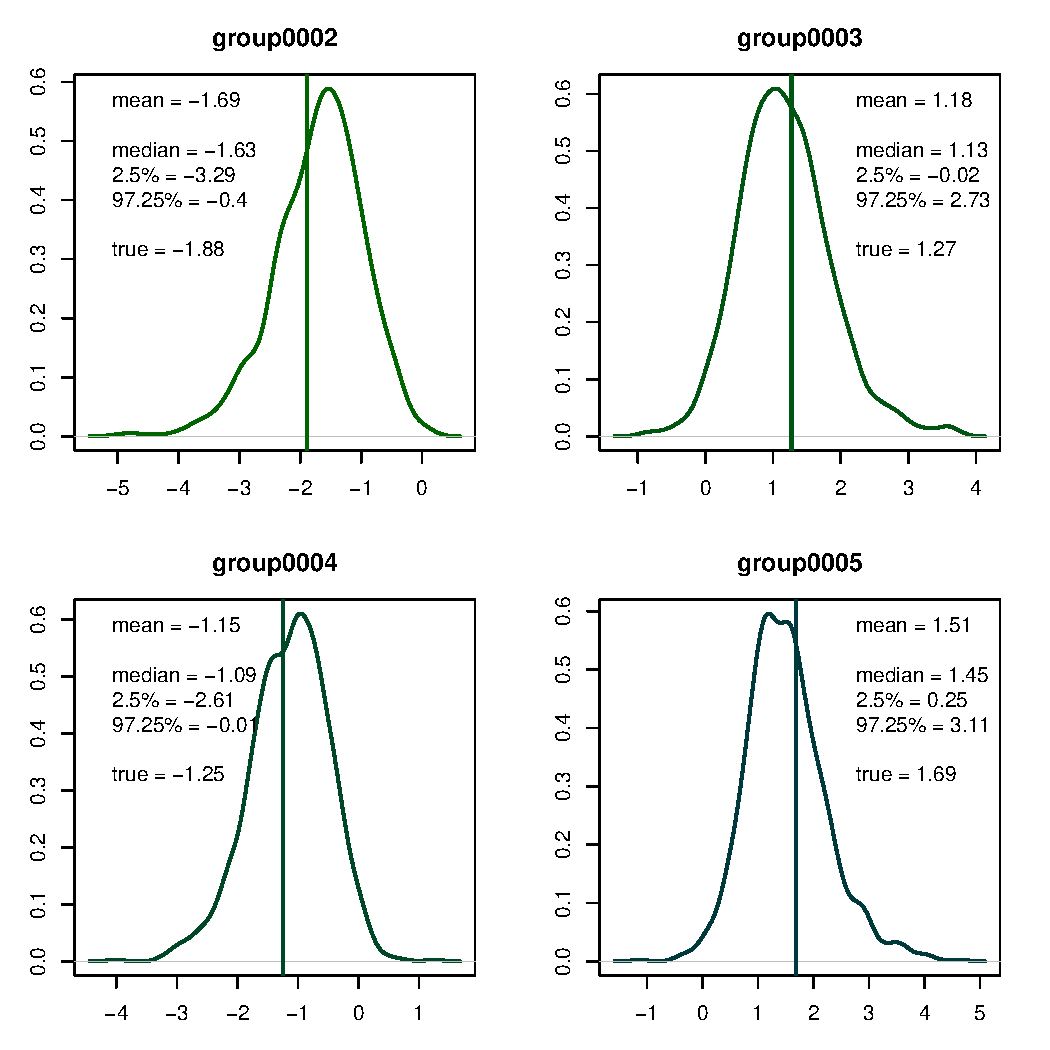
\includegraphics[width=0.6\textwidth]{graphics/glmmj5i20}
  \caption{Group levels in sample GLMM based on predicted random effect (conditional mode); 5 groups; 20 observations per group; 1,000 simulations; the horizontal line marks the true value}
  \label{fig:glmmj5i20}
\end{figure}
\begin{figure}[!htpb]
  \centering
  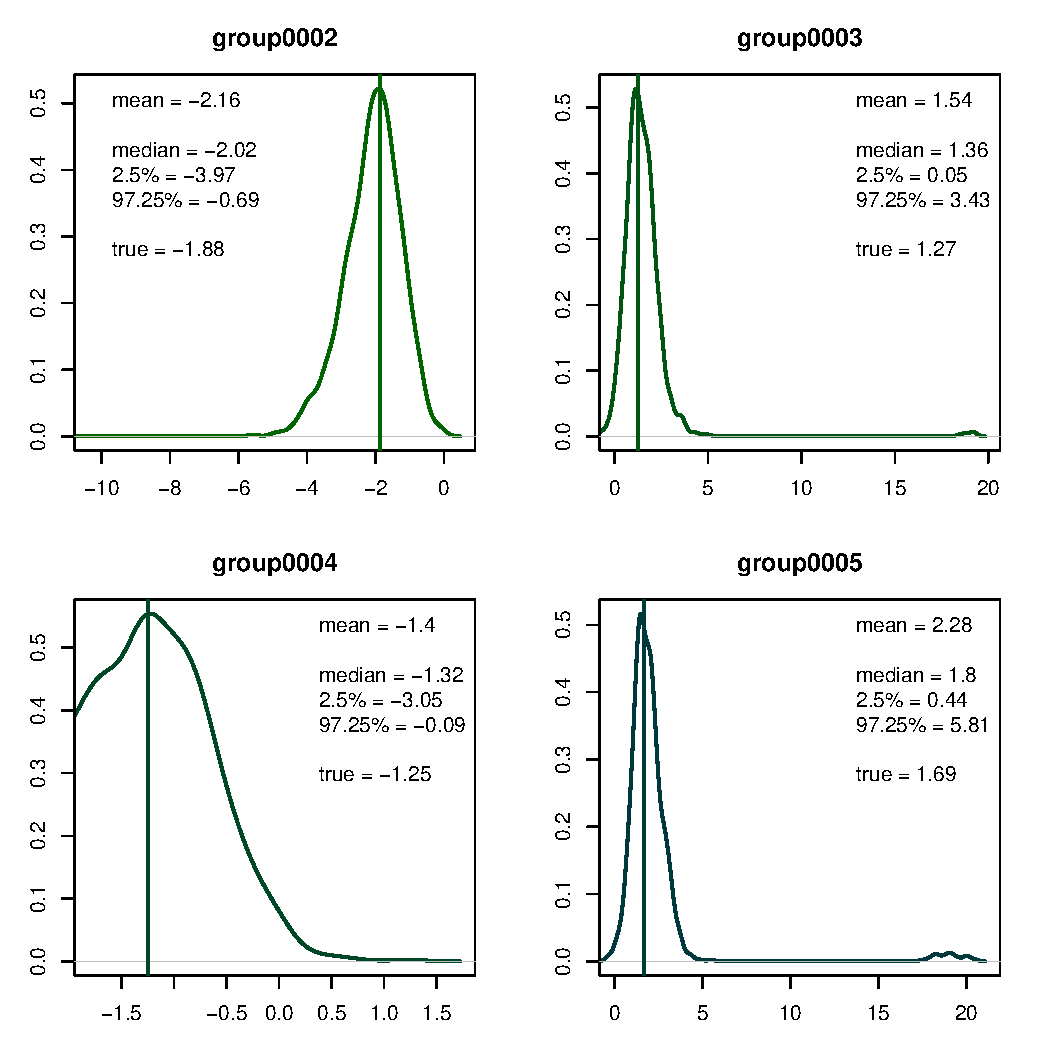
\includegraphics[width=0.6\textwidth]{graphics/glmj5i20}
  \caption{Estimated fixed effects for the grouping factor in sample GLM; 5 groups; 20 observations per level of the grouping factor; 1,000 simulations; the horizontal line marks the true value}
  \label{fig:glmj5i20}
\end{figure}

The per-group predictions lean slightly towards $0$ in the GLMM (Figure~\ref{fig:glmmj5i20}), but the fixed effects estimates in the GLM are prone to occasional misestimations.
While the overall spread is roughly the same for both approaches, the GLM estimates have massive outliers (down to approximately $-10$ and up to $20$), which leads to slightly larger 95\% percentile intervals.
In this scenario (crafted to work reasonably well with a fixed or a random effect), however, random and fixed effects lead to very similar results, albeit with different advantages and disadvantages.
More differences will be discussed in Sections~\ref{sec:significancetestingandcoefficientsofdetermination} and \ref{sec:morecomplexmodels}.


\subsubsection{Significance testing, model selection, and coefficients of determination}
\label{sec:significancetestingandcoefficientsofdetermination}

One commonly given reason to use a random effect is that ``the researchers are not interested in the individual levels of the random effect factor'' (or variations thereof).
Such recommendations should be taken with a grain of salt.
\citet[245--247]{GelmanHill2006} summarise the diverging and partially contradicting recommendations for what should be a random effect along with their motivations.
They conclude that there is essentially no principled conceptual or mathematical way of deciding what should be a random effect and what a fixed effect.
In this chapter, a more technical approach (which favours the solution that leads to the more robust model estimates) was therefore suggested.

However, it is not adequate to do any kind of significance test on the levels of the random effect because they are not estimates in the conceptual and technical sense.%
\footnote{Essentially, we do not assume them to be fixed population parameters, which would be the case for estimates such as fixed effects coefficients.}
% The conditional modes are not estimates, and only for estimates is significance testing a well-defined activity.
There are ways of calculating \textit{prediction intervals} (which are not the same as confidence intervals) for conditional modes in order to specify the quality of the fit (see Section~\ref{sec:specifyingmodelsusinglme4inr}), but they should not be misused for talking about significance.
% If this is absolutely required, fixed effects are the way to go.
Not doing significance tests for single levels of the grouping factor does, however, not mean that the researcher is not interested in the individual conditional modes, which is proven by the fact that they are often reproduced in research papers, for example in the form of a dot plot.
Also, the simulation in Section~\ref{sec:choosingbetweenrandomandfixedeffects} shows that we can use a random effect and still get a good idea of the per-group tendencies.
Additionally, a random effect allows the researcher to quantify the between-group variance, which is not possible in the same way with fixed effects.

A related question is \textit{model selection}, \ie whether the inclusion of the random effect improves the model quality.
It is recommended here to include all conceptually necessary random effects and only remove them if they have no effect.
To check whether this is the case, the estimated between-group variance is the first thing to look at.
If it is close to $0$, there is most likely not much going on between groups, or there simply was not enough data to estimate the variance.
In LMMs, it is possible to compare the residual (observation-level) variance with the between-group variance to see which one is larger, and to which degree.
If, for example, the residual variance is $\sigma_{\epsilon}=0.2$ and the between-group variance is $\sigma_{\alpha}=0.8$, then we can say that the between-group variance is four times larger than the residual variance, which would indicate a high importance of the random effect.
This comparison is impossible in GLMMs because their (several types of) residuals do not have the same straightforward interpretation as in LMMs.

Furthermore, models can be compared using likelihood ratio (LR) tests.
In such tests, a model including the random effect and a model not including it are compared, similar to LR tests for the comparison of fixed effects.
Such pairs of models, where one is strictly a simplification of the other, are called \textit{nested models} (not to be confused with \textit{nested effects} discussed in Section~\ref{sec:crossedandnestedeffects}).
A sometimes more robust alternative to the ordinary LR test are parametric bootstrap tests (see also Section~\ref{sec:specifyingmodelsusinglme4inr}).
With all this, it should be kept in mind that it is \textit{never} appropriate to compare a GLMM with a random effect and a GLM with the same factor as a fixed effect using any test or metric (including so-called information criteria such as Akaike's or Bayes').

Coefficients of determination (pseudo-$R^2$) can be used to give some idea of the overall model fit.
%should not be used for model selection, because they usually do not penalise complexity enough (\ie the pseudo-$R^2$ measures rise with added complexity).
%They can still be used to give some idea of the model fit, however.
For GLMMs, \citet{NakagawaSchielzeth2013} have proposed a method that distinguishes between \textit{marginal} $R^2$ (only fixed effects) and \textit{conditional} $R^2$ (fixed and random effects).
This has become a de facto standard, and we now show its consistency with Nagelkerke's $R^2$ for GLMs.
Using the simulated data described in the last section, Figures~\ref{fig:rsqglmmj5i20} and \ref{fig:rsqglmj5i20} show that the marginal $R^2$ for a GLMM estimate is roughly the same as Nagelkerke's $R^2$ for a GLM estimate where the grouping factor is ignored.
Also, the conditional $R^2$ for a GLMM estimate is roughly the same as Nagelkerke's $R^2$ for a GLM estimate which includes the grouping factor as a fixed effect.
It should be noted that the simulations were explicitly designed such that the grouping factor (five levels with enough observations per level) could be used successfully as a fixed effect or a random effect, which is usually not the case with real data.

\begin{figure}[!htpb]
  \centering
  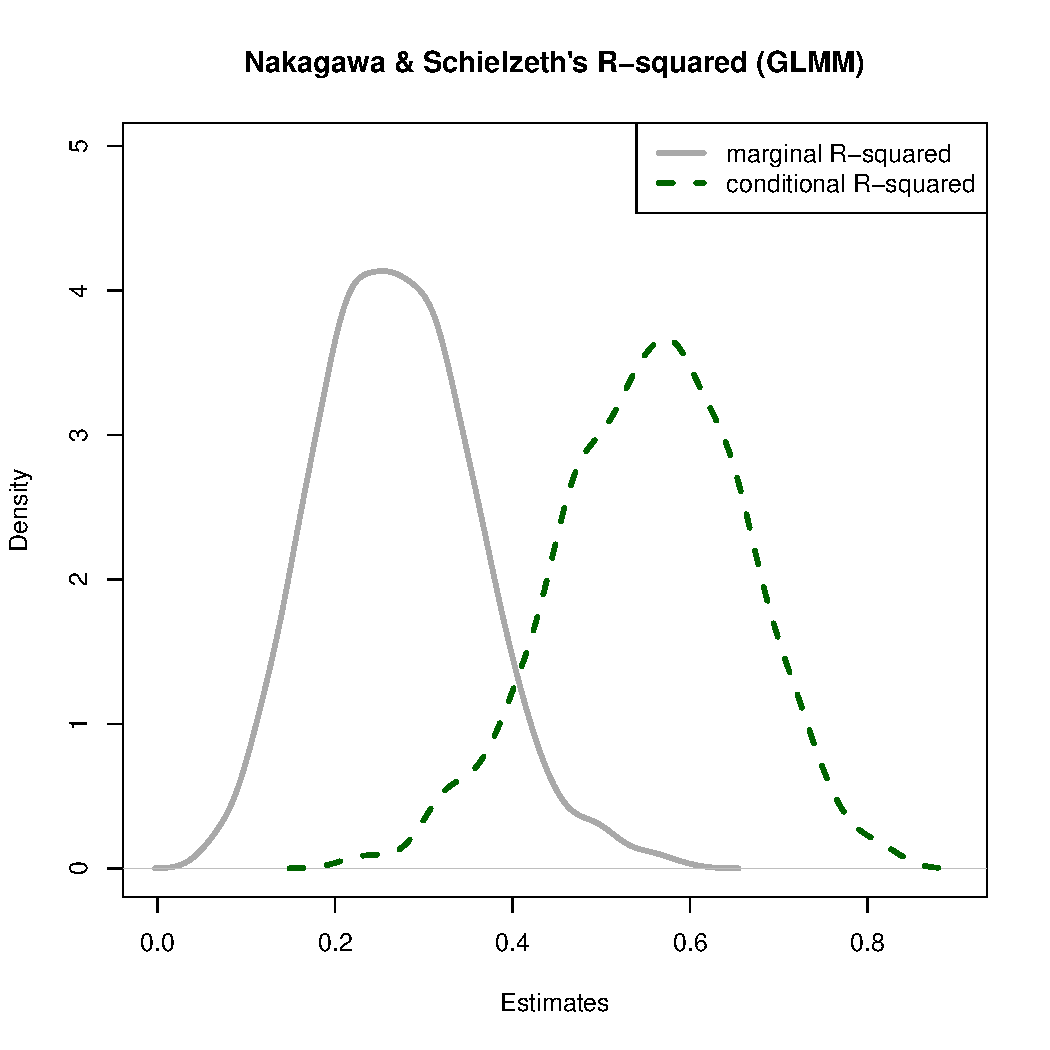
\includegraphics[width=0.6\textwidth]{graphics/rsqglmmj5i20}
  \caption{Distribution of Nakagawa \& Schielzeth's $R^2$ in the simulations described in Section~\ref{sec:choosingbetweenrandomandfixedeffects}}
  \label{fig:rsqglmmj5i20}
\end{figure}

\begin{figure}[!htpb]
  \centering
  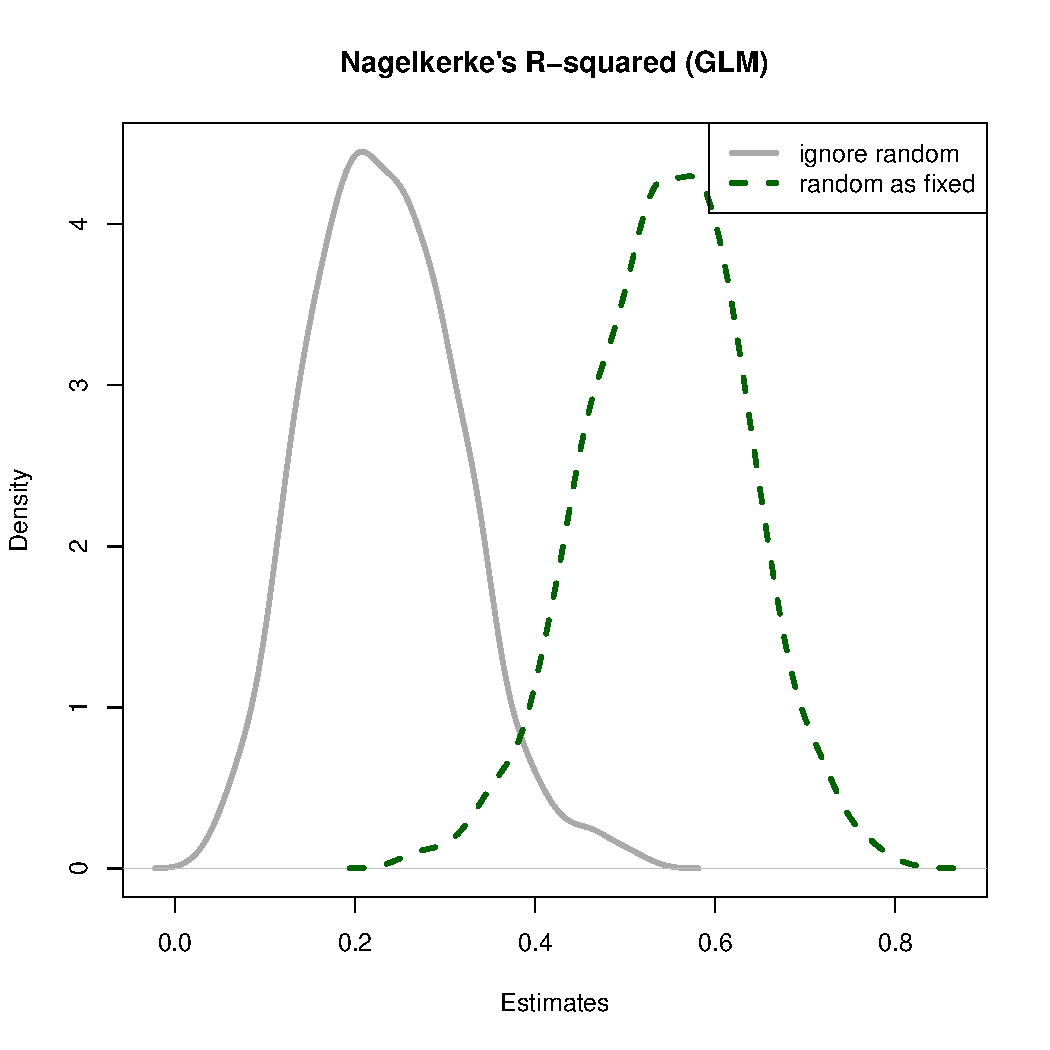
\includegraphics[width=0.6\textwidth]{graphics/rsqglmj5i20}
  \caption{Nagelkerke's $R^2$ in the simulations described in Section~\ref{sec:choosingbetweenrandomandfixedeffects} for a GLM that ignores the grouping factor and a model that includes it as a fixed effect}
  \label{fig:rsqglmj5i20}
\end{figure}

\subsubsection{More complex models}
\label{sec:morecomplexmodels}

% This section shows briefly how more complex models are specified before Section~\ref{sec:specifyingmodelsusinglme4inr} demonstrates how models are estimated in \texttt{R}, including interpretations of the output.

\paragraph{Varying intercepts and slopes}

While it is possible to have just a varying slope, this is rarely useful, and we discuss only varying-intercept and varying-slope (VIVS) models.
An example of when a VIVS model might be useful was given in Section~\ref{sec:randominterceptsandslopes}, and readers might want to review this before continuing on.
We extend the simple model from (\ref{eq:glmm01}), and the fixed effect coefficients for which a random slope is specified simply receive group indices; see (\ref{eq:glmm05}).
Instead of estimating a fixed coefficient, coefficients are predicted and assumed to come from a random (normal) distribution.
We use $\beta_{d:l}$ to denote the coefficient for givenness varying by lemma.

\begin{equation}
  P(y^i=1)=logit^{-1}(\alpha_{l}^{j[i]}+\beta_{d:l}^{j[i]}\cdot x_d^i)
  \label{eq:glmm05}
\end{equation}

A source of problems in VIVS models is the fact that in addition to the variance in the intercepts and slopes, the covariance between them has to be estimated.
If in groups with a higher-than-average intercept, the slope is also higher than average, they are positively correlated, and vice versa.
These relations are captured in the covariance.
Condition (\ref{eq:glmm06}) is added, where the indices $l$ and $d:l$ are omitted for readability.

\begin{equation} 
  \left( \begin{smallmatrix} \alpha^j \\ \beta^j \end{smallmatrix}\right) \sim
    \left(
    \left( \begin{smallmatrix} \mu_{\alpha}\vphantom{\beta^j} \\ \mu_{\beta}\vphantom{\beta^j} \end{smallmatrix} \right), 
      \left( \begin{smallmatrix} \sigma_{\alpha}^2 & \rho\sigma_{\alpha}\sigma_{\beta} \\
	\rho\sigma_{\alpha}\sigma_{\beta} & \sigma_{\beta}^2 \end{smallmatrix} \right)
    \right)
  \label{eq:glmm06}
\end{equation}

(\ref{eq:glmm06}) says that the joint distribution of the intercepts $\alpha^j$ and the slopes $\beta^j$ follows a bivariate normal distribution with means $\mu_{\alpha}$ and $\mu_{\beta}$.
The variance in the intercepts is $\sigma_{\alpha}$, the variance in the slopes is $\sigma_{\beta}$, and the coefficient for the covariance between them is $\rho$.
Figure~\ref{fig:multnorm} shows the bivariate density distributions for two (1) negatively correlated, (2) non-correlated, and (3) positively correlated normally distributed variables.

\begin{figure}[!htpb]
  \centering
  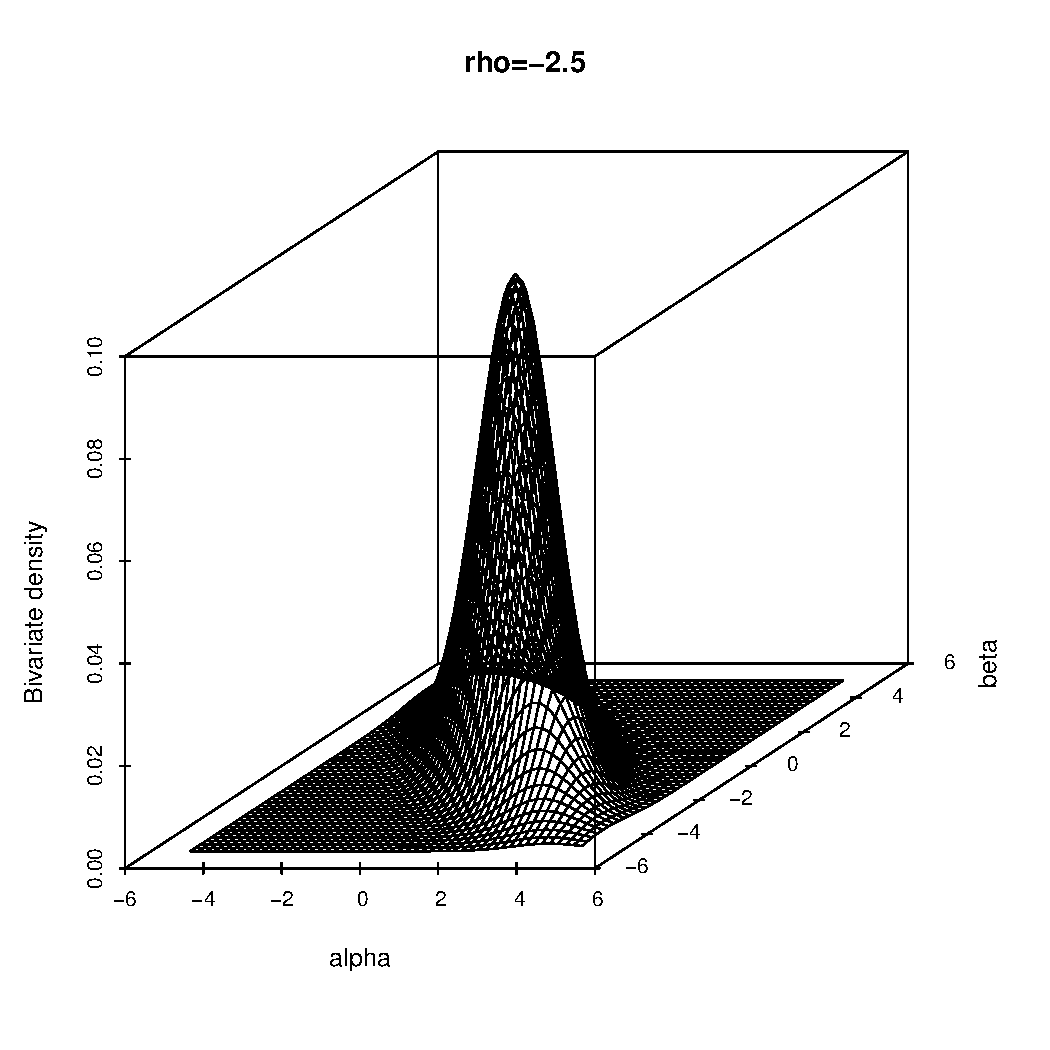
\includegraphics[width=0.33\textwidth]{graphics/multnorm1}~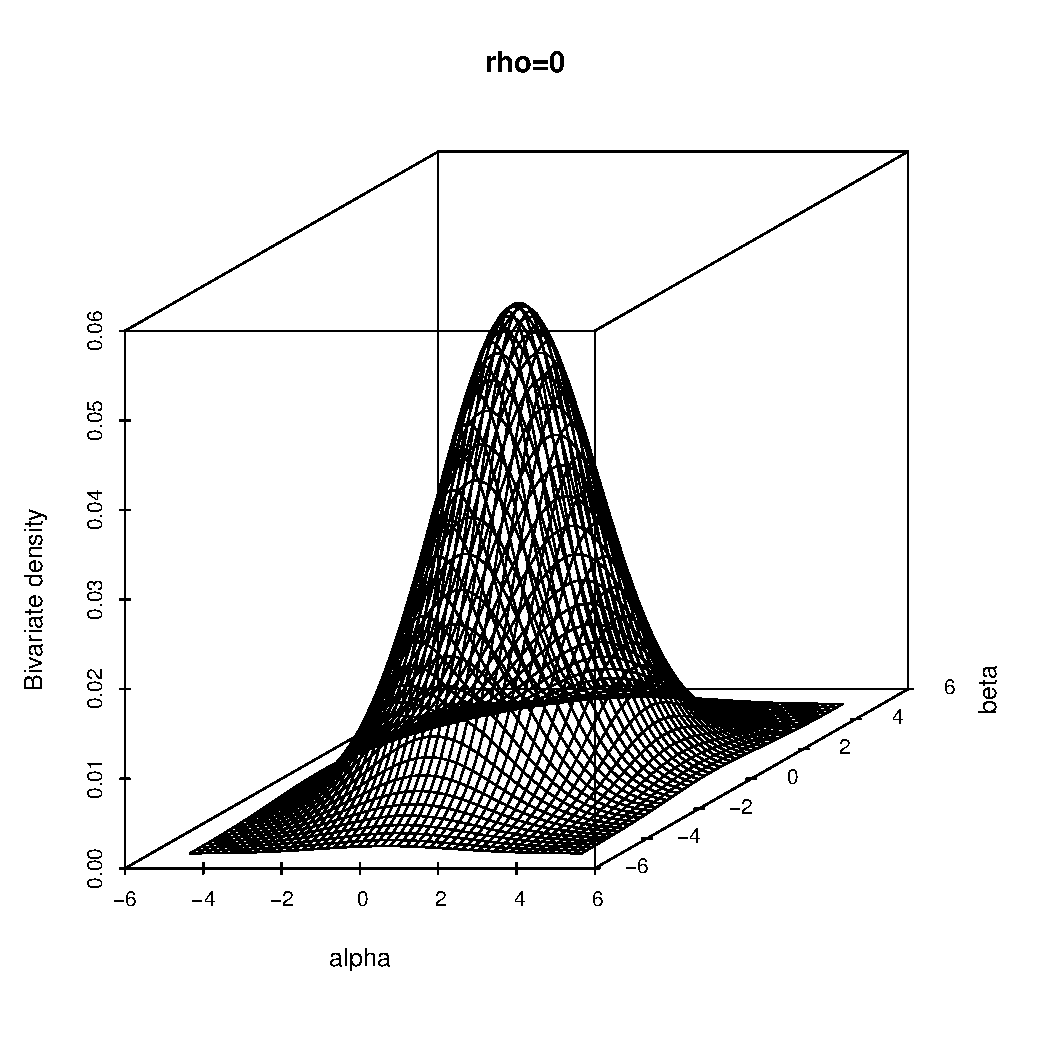
\includegraphics[width=0.33\textwidth]{graphics/multnorm2}~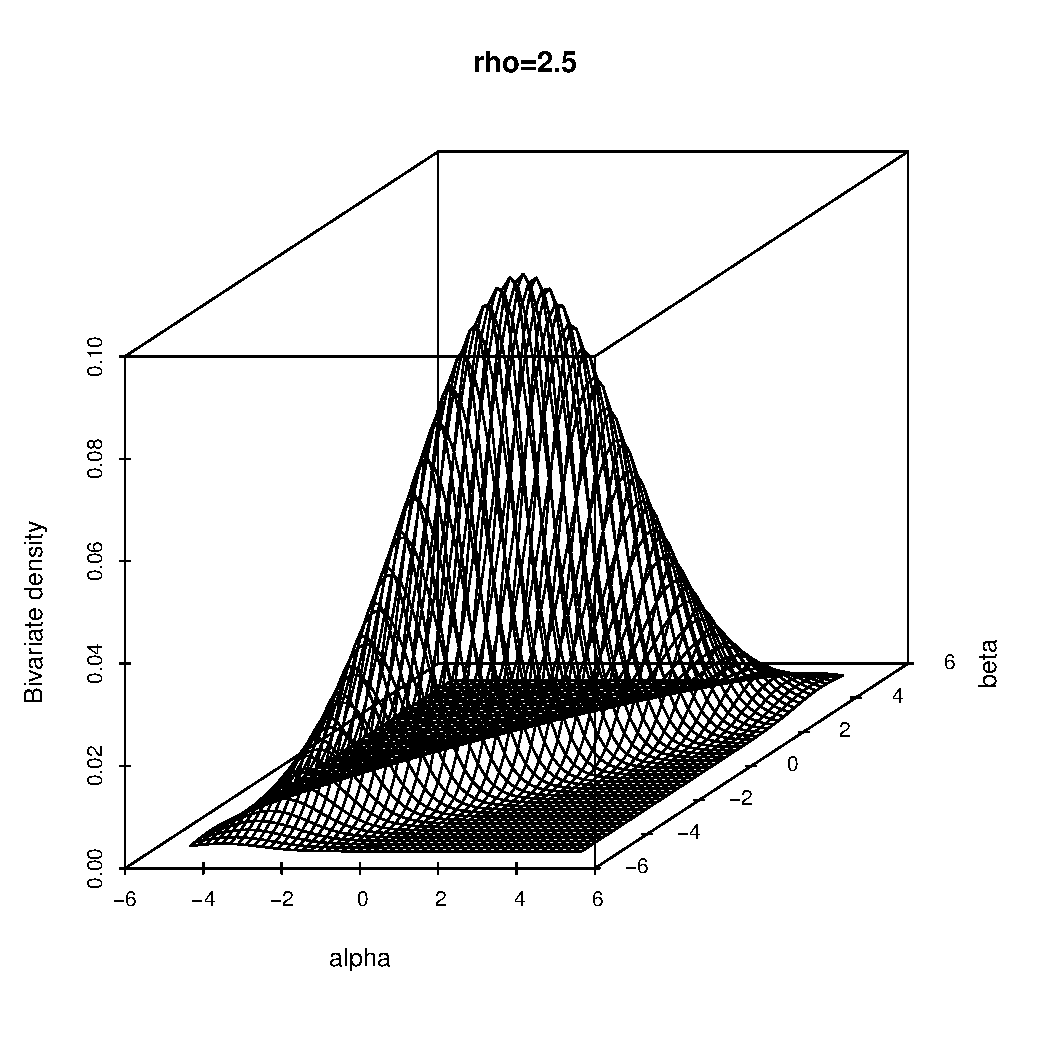
\includegraphics[width=0.33\textwidth]{graphics/multnorm3}
  \caption{Bivariate normal density distribution with different correlation coefficients $\rho$; $\sigma_{\alpha}=\sigma_{\beta}=3$; $\mu_{\alpha}=\mu_{\beta}=0$}
  \label{fig:multnorm}
\end{figure}

The number of variance parameters to be estimated thus obviously increases with more complex model specifications, and the estimation of the parameters in the presence of complex variance-covariance matrices requires considerably more data than estimating a single variance parameter.
The estimator might converge, but typically covariance estimates of $-1$ or $1$ indicate that the data was too sparse for a successful estimation of the parameter.
In this case, the model is \textit{over-parametrised} and needs to be simplified.
% In Section~\ref{sec:afterfittingmodelswithlme4}, it will be shown how to interpret the \texttt{lme4} output appropriately.

\paragraph{Nested and crossed random effects}

As it was explained in Section~\ref{sec:crossedandnestedeffects}, nested random effects are adequate when grouping factors are nested within other grouping factors.
Technically, while varying slopes can be understood as interactions between a fixed and a random effect, nested random intercepts can be understood as interactions between two or more random effects.
Crossed random effects are just several unrelated random effects.
(\ref{eq:glmm07}) shows the model specification, extending (\ref{eq:glmm01}) with a varying intercept $\alpha_s$.
This could be for example semantic classes which nest individual lemmas.
It could also be another grouping factor for speaker, completely unrelated to the lemmas.

\begin{equation}
  P(y^i=1)=logit^{-1}(\alpha_{s}^{k[i]}+\alpha_{l}^{j[i]}+\beta_d\cdot x_d^i)
  \label{eq:glmm07}
\end{equation}

The difference is that in the nested case, $k[i]=k[j]$, \ie the level of the nesting factor can be selected based on the nested factor as well as based on the single observation.
As was mentioned in Section~\ref{sec:crossedandnestedeffects}, the question is rather one of how the way the data are organised.
% In the model specification, there are no obvious differences.

\paragraph{Second-level predictors}

In Section~\ref{sec:hierarchicalormultilevelmodels}, situations were introduced where the random effects themselves can be partially predicted from fixed-effects.
In this case, an additional linear model is specified for the random effect instead of the simple normal distribution predictor.
We extend (\ref{eq:glmm01}) by a predictor $\gamma_f$ for the lemma frequency.
The lemma frequencies themselves we denote by $u_f$, and we index them with $j$, just like the verb lemmas.
This is reasonable because for each verb lemma, there is exactly one frequency.
The first-level model specification remains the same, namely (\ref{eq:glmm08}).

\begin{equation}
  P(y^i=1)=logit^{-1}(\alpha_{l}^{j[i]}+\beta_d\cdot x_d^i)
  \label{eq:glmm08}
\end{equation}

However, instead of (\ref{eq:glmm02}), the varying intercept is predicted from (\ref{eq:glmm09}).

\begin{equation}
  \alpha_l^j\sim N(\gamma_0+\gamma_f\cdot u_f^j,\sigma_l^2)
  \label{eq:glmm09}
\end{equation}

Instead of just the mean of the $\alpha_j$ values, the model in (\ref{eq:glmm09}) specifies a second-level intercept $\gamma_0$ and a second-level fixed coefficient $\gamma_f$.
% If the lemma frequency plays a role, this approach can lead to a more precise prediction of the varying first-level intercept compared to the less elaborate approach in (\ref{eq:glmm02}).
% True multilevel models increase the complexity of GLMMs, especially if third-level models, fourth-level models, etc. are used.
% Situations for multilevel modeling are quite frequently encountered, however.
% Especially when it comes to speakers as random effects, the age, the gender, the region of birth (if this grouping factor has too few levels to be used as a random effect nesting speakers), etc.\ are ideal second-level predictors.
% The \texttt{lme4} syntax treats second-level predictors like interactions between a fixed and a random effect, see also Section~\ref{sec:specifyingmodelsusinglme4inr}.

% Readers finding it difficult to see why (\ref{eq:glmm09}) is a plain linear model could consider the equivalent formulation in (\ref{eq:glmm10}) and (\ref{eq:glmm11}).
%  
% \begin{align}
%   \alpha_l^j   =    & \gamma_0+\gamma_f\cdot u_j^j+\epsilon_l^j \label{eq:glmm10}\\
%   \epsilon_l^j \sim & N(0, \sigma^2) \label{eq:glmm11}
% \end{align}

\paragraph{Remarks on models for longitudinal studies}

A longitudinal study is one wherein single subjects (usually speakers) are observed at different points in time, for example second-language learners after different years of learning a second language.
% This section briefly discusses the main points to consider when such models -- which can get quite complex -- are specified.
First, the observations are grouped by the individual speakers.
It is thus recommended to include the speaker grouping factor, typically as a random effect.
% either as a fixed effect (up to five speakers) or random effect (more speakers).
Second, there might be time parameters such as years of learning.
% Third, the errors might be correlated.

We now assume we have a (fictional) sample from a learner corpus of German as a second language.
In a logistic regression, we examine whether Swedish and English learners use the weak form or the strong forms of attributive adjectives in NPs with a determiner.
The crucial morpho-syntactic variable is whether the determiner has itself a strong ending or not.
An example of a strong adjective is seen in \textit{ein großer Apfel} `a large apple', an example of a weak adjective in \textit{der große Apfel} `the large apple'.
We include an appropriate first-level term which encodes the choice of ending on the determiner $\beta_d\cdot x_d^i$ in the model.
A random effect for individual learners is also included as $\alpha_l^{j[i]}$.
Additionally, we add a term for the number of years the learners have learned German.
% (potentially logarithmised or otherwise transformed).
However, since learners progress with different speed, a random slope is indicated, and the term becomes $\beta_{y:l}^{j[i]}\cdot x_y^i$.
The first-level model is thus (\ref{eq:glmm013}).

\begin{equation}
  P(y^i=1)=logit^{-1}(\alpha_l^{j[i]} + \beta_d\cdot x_d^i + \beta_{y:l}^{j[i]}\cdot x_y^i)
  \label{eq:glmm013}
\end{equation}

The main purpose of our study might be to find out whether Swedish and English learners differ with respect to the phenomenon at hand.
Therefore, the first language is added as a second-level predictor with the term $\gamma_f\cdot u_f^j$, where $u_f^j$ is $1$ if the language of learner $j$ is Swedish, and $0$ if it is English.
Since we have a random intercept and a random slope we need to distinguish between $\gamma_f^{\alpha}\cdot u_f^j$ for the random intercept and $\gamma_f^{\beta}\cdot u_f^j$ for the random slope.
The second level model to go with (\ref{eq:glmm013}) is therefore (\ref{eq:glmm14}).

\begin{equation} 
  \left( \begin{smallmatrix} \alpha^j \\ \beta^j \end{smallmatrix}\right) \sim
    \left(
    \left( \begin{smallmatrix} \gamma_0^{\alpha}+\gamma_f^{\alpha}\cdot u_f^j \\ \gamma_0^{\beta}+\gamma_f^{\beta}\cdot u_f^j    \end{smallmatrix} \right), 
      \left( \begin{smallmatrix} \sigma_{\alpha}^2 & \rho\sigma_{\alpha}\sigma_{\beta} \\
	\rho\sigma_{\alpha}\sigma_{\beta} & \sigma_{\beta}^2 \end{smallmatrix} \right)
    \right)
  \label{eq:glmm14}
\end{equation}

Although this is a quite complex model already, there might be more problems.
The performance of learners after $n+1$ years of learning is usually correlated to a high degree with their performance after $n$ years.
This can lead to \textit{autocorrelation} in the errors, violating basic modeling assumptions.
To take care of this, model which allow for explicitly specified error structures must be used.
Anyone wishing to use such models should consult further references (\eg \citealt{Fox2016} and \citealt{ZuurEa2009}).

